\documentclass[a4paper]{article}
\usepackage[utf8]{inputenc}
\usepackage[italian]{babel}
\usepackage{titling}
\usepackage{graphicx}
\usepackage{wrapfig}
\usepackage{float}
\usepackage{amsmath}
\usepackage{listings}
\usepackage[table,xcdraw]{xcolor}
\usepackage[numbers]{natbib}
\usepackage{amssymb}
\renewcommand{\bibfont}{\small}

\newcommand{\subtitle}[1]{%
	\posttitle{%
		\par\end{center}
	\begin{center}\large#1\end{center}
	\vskip0.5em}%
}

\begin{document}

%opening
\title{Studio sulla Stabilità dei Dischi di Accrescimento di Shakura \& Sunyaev}
\subtitle{Appunti}
\author{Riccardo Aurelio Gilardi}
\maketitle

\newpage
\tableofcontents
\newpage

\section{Introduzione}
Lo scopo di questa tesi vuole essere quello di riassumere ed approfondire le teorie sulla stabilità delle regioni interne dei dischi di accrescimento, nel contesto del modello introdotto da Shakura e Sunyaev nel loro articolo del 1973 ~\cite{ShakuraSunyaev1973}.

Per mantenere una descrizione più semplice e meno dispersiva, ho deciso di lavorare seguendo l'esempio di molti autori, analizzando un sistema formato da una stella ordinaria e un buco nero. Questa scelta è guidata dal fatto che il materiale in accrescimento non risente di effetti legati alla relatività generale a distanze maggiori di tre volte il raggio di Scwartzchild del buco nero
\footnote{166FKR}
e, al contrario del caso di accrescimento intorno a una stella a neutroni, il sistema in accrescimento al buco nero non sarà interessato da fenomeni legati ai campi magnetici e alla torsione che essi possono applicare al materiale in accrescimento.

La scelta è anche giustificata dal fatto che, nonostante i buchi neri che fanno parte di sistemi binari siano meno semplici da osservare rispetto, per esempio, di quelli contenenti nane bianche, la loro estrema compattezza permette di apprezzare il comportamento del disco nelle sue regioni più interne.

Prima di parlare delle instabilità nei dischi, comincerò introducendo i concetti e le formule che descrivono un disco di accrescimento, la fisica che lo governa e il suo stato stazionario.

\newpage
\section{Accrescimento in sistemi binari}
L'accrescimento è uno dei processi di conversione di massa in energia tra i più efficienti nell'universo, che si sviluppa in sistemi binari di cui almeno un membro è un corpo compatto: una nana bianca, una stella a neutroni o un buco nero.

Le cause scatenanti del trasporto di materiale tra due membri di un sistema binario possono essere un travalicamento da parte di uno dei membri del sistema del suo lobo di Roche o la cattura gravitazionale da parte del corpo compatto di venti stellari emessi dal suo compagno.

Il primo di questi due processi è sicuramente meglio descritto e più semplice da trattare analiticamente e permette di dedurre delle informazioni interessanti sulla forma della viscosità, il meccanismo con cui viene trasportato momento angolare e che rende possibile l'accrescimento.

\subsection{Deflusso attraverso i Lobi di Roche}
	Edouard Roche ricavò la forma della struttura che prende il suo nome studiando l'orbita dei satelliti planetari. Lo fece descrivendo il moto di alcune particelle di test immerse in un potenziale gravitazionale generato da due corpi orbitanti intorno alla loro reciproca attrazione gravitazionale.
	
	La sua costruzione è essenziale e piuttosto elegante e si può ricavare partendo da poche semplici ipotesi, prima di calcolarne numericamente i parametri: la particella di test deve avere massa abbastanza piccola, al confronto con quella dei due corpi massicci, da non poterne influenzare in modo rilevante l'orbita; le orbite sono da considerarsi kepleriane e circolari, questo non è sempre vero in pratica, ma in generale le forze mareali tendono a rendere circolari orbite eccentriche in tempi scala molto minori di quelli caratteristici di un meccanismo di trasporto di materia; infine le masse sono da considerarsi condensate nel loro centro.
	
	Per descrivere qualsiasi flusso di gas tra i due corpi del sistema ha senso utilizzare l'\textit{equazione di Eulero} in un sistema di riferimento co-rotante col sistema binario, con velocità angolare $\omega$ rispetto al sistema inerziale. Questo comporta la presenza nell'equazione di termini che tengano conto delle forze centrifughe e di quelle di Coriolis ($-2\omega\times\textbf{v}$), così da ottenere:
	\begin{equation}
		\frac{\partial \textbf{v}}{\partial t}+(\textbf{v}\cdot\nabla)\textbf{v}=-\nabla\Phi_R-2\omega\times\textbf{v}-\frac{1}{\rho}\nabla P
	\end{equation}
	Con $\omega$ parallela al versore ortogonale al piano orbitale $\textbf{e}$:
	\begin{equation}
		\omega=\left[\frac{G(M_1+M_2)M_\odot}{a^3}\right]^{1/2}\textbf{e}
	\end{equation}
	e $\Phi_R$ il \textit{Potenziale di Roche}, che contiene i termini relativi all'attrazione gravitazionale e le forze centrifughe:
	\begin{equation}
		\Phi_R(\textbf{r})=-\frac{GM_1M_\odot}{\vert\textbf{r}-\textbf{r}_1\vert}-\frac{GM_2M_\odot}{\vert\textbf{r}-\textbf{r}_2\vert}-\frac{1}{2}(\omega\times\textbf{r})^2
	\end{equation}
	
	\begin{figure}[H]
		\centering
		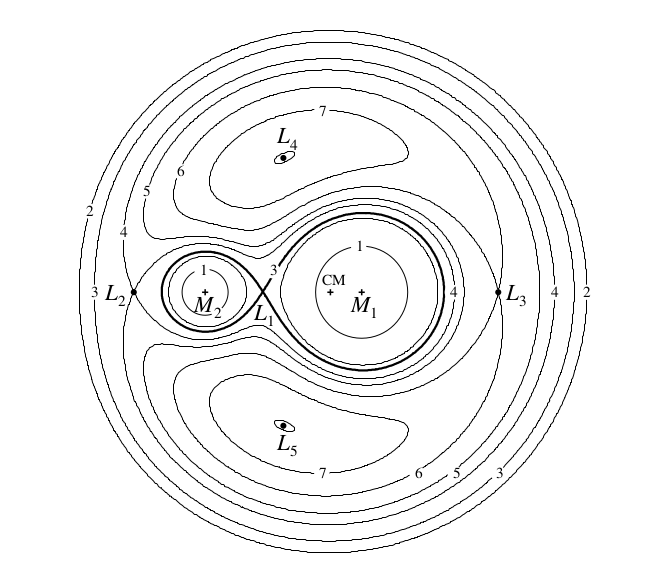
\includegraphics[width=0.6\linewidth]{RocheEquipotential}
		\caption{Una rappresentazione della sezione dei lobi e delle curve equipotenziali. $L_1$ è il punto lagrangiano interno}
		\label{fig:rocheequipotential}
	\end{figure}
	
	Le curve equipotenziali di $\Phi_R$ dipendono solo dal rapporto fra le masse $q=\frac{M_2}{M_1}$ e la loro scala dipende dalla distanza che le separa $a$. Per $q\sim1$ i lobi saranno simmetrici, mentre per rapporti $q<<1$ o $q>>1$ avranno volumi diversi.
	
	Per distanze sufficientemente alte, la forma delle curve equipotenziali corrisponde a quella di una singola massa $M=(M_1+M_2)M_\odot$, mentre a distanze brevi il potenziale è dominato da quello della stella più vicina. Le buche di potenziale centrate sulle posizioni dei due corpi $\textbf{r}_1$ e $\textbf{r}_2$, sono separate dalla cosiddetta \textit{superficie critica}.
	
	Il punto separatore dei due lobi, detto \textit{punto lagrangiano interno} è una sella per $\Phi_R$ tale che se del materiale in uno dei due lobi si trovasse in sua prossimità (magari a seguito dell'espansione della stella da cui proviene, che si ritroverà ad occupare tutto il volume del suo lobo), passerebbe attraverso lui verso il lobo della compagna, piuttosto che attraversare la superficie critica del potenziale.
	
	Si può trattare in maniera quantitativa la stima della geometria dei lobi e sul trasporto di materia, ricavando quindi la loro dipendenza da $q$ ed $a$. Qualcosa che è interessante osservare è che questi due termini varieranno nel tempo durante qualsiasi processo di accrescimento, comportando una contrazione del lobo del corpo che sta cedendo massa ed una riduzione del periodo orbitale del sistema, insieme alla riduzione della distanza tra i due corpi, dovuta al processo di trasferimento del momento angolare nel sistema.
	
	Si può dimostrare che, nell'ipotesi di accrescimento lento e totale $\dot{M}_1+\dot{M}_2=0$, il trasferimento di materia tra i due lobi si svolge nello stesso tempo scala con cui il momento angolare viene perso.
	
	Ipotizzando sia $M_2$ a cedere materia a $M_1$ e con $J$ momento angolare totale del sistema, abbiamo che:
	
	\begin{equation}
		-\frac{\dot{M}_2}{M_2}=\frac{-\dot{J}/J}{4/3-M_2/M_1}
	\end{equation}
	
	e analogamente si trova che

	\begin{equation}
		\frac{\dot{a}}{a}=2\frac{\dot{P}}{3P}=\frac{2\dot{J}/3J}{4/3-q}
	\end{equation}
	
\subsection{Formazione di un disco}
	Il trasporto di materia attraverso i lobi implica che il materiale trasportato sarà dotato di un momento angolare non indifferente, che non gli permetterebbe di essere accresciuto direttamente dall'altra stella.
	
	Se il periodo orbitale del sistema non è molto lungo, il lobo a cui viene accresciuta la materia, la vedrà provenire dal punto lagrangiano con velocità quasi completamente ortogonale alla linea dei centri che unisce le due masse. 
	
	Se definisco $b_1$ la distanza tra $M_1$ e $L_1$, posso approssimare il valore della componente istantaneamente ortogonale alla linea dei centri della velocità in un sistema di riferimento inerziale
	\begin{equation}
		v_\perp\sim b_1\omega\sim 100\,M_1^{1/3}(1+q)^{1/3}P^{-1/3}_{day}\,km\,sec^{-1}
	\end{equation}  
	Mentre per la componente parallela, poiché immagino la forza che permette il passaggio tra i lobi della materia sia legata alla pressione, posso supporre valga
	\begin{equation}
		v_\parallel \lesssim c_{s_2}
	\end{equation}
	con $c_{s_2}$ velocità del suono nel lobo secondario, da cui proviene la materia e poiché nel mezzo interstellare $T\lesssim10^5$ e per un gas vale $c_s\cong10(T/10^4\,K)^{1/2}km\,sec^{-1}$, deve essere $v_\parallel\lesssim10\,km\,sec^{-1}$
	
	Quindi in totale il moto del materiale in accrescimento a $M_1$ deve essere supersonico 

\subsection{Viscosità}

\newpage
\section{Modello Stazionario di Dischi di Accrescimento}
\subsection{Il modello di Shakura e Sunyaev}
\begin{equation}
	\nu=\alpha c_sH
\end{equation}
\begin{equation}
	\begin{cases}
		\Sigma=5.2\alpha^{-4/5}\dot{M}_{16}^{3/20}M^{1/4}_1R_{10}^{-3/4}f^{14/5}\,g\,cm^{-2}\\
		H=1.7\times10^8\alpha^{-1/10}\dot{M}^{3/20}_{16}M^{-3/8}_1R_{10}^{9/8}f^{3/5}\,cm\\
		\rho=3.1\times10^{-8}\alpha^{-7/10}\dot{M}^{11/20}_{16}M^{5/8}_1R_{10}^{-15/8}f^{11/5}\,g\,cm^{-3}\\
		T_c=1.4\times10^{4}\alpha^{-1/5}\dot{M}^{3/10}_{16}M^{1/4}_1R_{10}^{-3/4}f^{6/5}\,K\\
		\tau=33\alpha^{-4/5}\dot{M}^{1/5}_{16}f^{4/5}\\
		\nu=1.8\times10^{14}\alpha^{4/5}\dot{M}^{3/10}_{16}M^{-1/4}_1R_{10}^{3/4}f^{6/5}\,g\,sec^{-1}\\
		\nu_R=2.7\times10^{14}\alpha^{4/5}\dot{M}^{3/10}_{16}M^{-1/4}_1R_{10}^{-1/4}f^{-14/5}\,cm\,sec^{-1}\\
	\end{cases}
\end{equation}
	con $f=\left[1-\left(\frac{R_*}{R}\right)^{1/2}\right]^{1/4}$ e $\dot{M}_{16}=\frac{\dot{M}}{(10^{16}\,g\,sec^{-3})}$
\newpage
\section{Evoluzione temporale dei dischi e instabilità}
\subsection{La derivazione di Lightman e Eardley}
\subsection{Instabilità termica e viscosa}
\subsection{Considerazioni sull'espressione della viscosità}
\subsection{Spettro di emissione}

\newpage

\renewcommand{\bibpreamble}{Per regioni di coerenza interna al testo e di visione ordinata degli argomenti, ho cercato di affrontarli seguendo il più delle volte la traccia e le argomentazioni come sono presentatate sul testo di \textit{Frank, King e Raine}~\cite{FrankKingRaineAccretionPower}, manuale di riferimento per quanto riguarda le teorie dell'accrescimento.
	
	Sono stati fondamentali anche alcune  \textit{review} di \textit{King}~\cite{King2012} e \textit{Pringle}~\cite{Pringle1981}, che sintetizzano efficacemente l'argomento dell'accrescimento e permettono di avere una visione di insieme dei risultati ottenuti.
	
	E' stato fondamentale per la mia comprensione dello sviluppo delle teorie, l'analisi e la lettura degli articoli originali sui modelli di disco di accrescimento intorno ai corpi compatti.
	Ho lavorato quindi anche con gli articoli seminali di \textit{Pringle}, \textit{Reese}, \textit{Shakura}, \textit{Sunyaev} e \textit{Pacholczyk}~\cite{PringleReese1972}~\cite{PringleReesePacholczyk1973}~\cite{ShakuraSunyaev1973} e la splendida analisi del lavoro nella fondazione della teoria di accrescimento di Zeldovich svolta da Shakura quest'anno~\cite{ShakuraZeldovich2018}.
	
	Per quanto riguarda in particolare l'argomento della tesi, ovvero l'instabilità nelle regioni dominate dalla pressione radiativa nel modello del disco di accrescimento, ho fatto riferimento al primissimo lavoro a riguardo di \textit{Lightman} ed \textit{Eardley}~\cite{LightmanEardley1974} e ad articoli successivi che estendono, propongono alternative, ne analizzanoi risultati o li computano. Questi sono stati scritti da \textit{Shakura} e \textit{Sunyaev}~\cite{ShakuraSunyaev1976}, \textit{Shapiro} con gli stessi \textit{Lightman} ed \textit{Eardley}~\cite{ShapiroLightmanEardley1976}, \textit{Taam} e \textit{Lin}~\cite{TaamLin1984} e \textit{Teresi}, \textit{Molteni} e \textit{Toscano}~\cite{TeresiMolteniToscano2004}.
	
	Per tutti gli aspetti non strettamente legati all'accrescimento ho fatto riferimento a tre manuali: il \textit{Maoz}~\cite{MaozNutshell} e il \textit{Prialnik} ~\cite{PrialnikStellarStructureEvolution} per i cenni sulla struttura dei corpi compatti e il \textit{Ghisellini}~\cite{GhiselliniRadiativi} per quanto riguarda i processi radiativi.}

\begin{thebibliography}{9}
	\bibitem{FrankKingRaineAccretionPower} 
	J. Frank, A. King, D. Raine
	"Accretion Power in Astrophysics"\\
	\textit{Cambridge University Press}, 2002 (III ed.)
	
	\bibitem{King2012} 
	A. King 
	"Accretion Disc Theory since Shakura and Sunyaev"\\
	\textit{arXiv}: 1201.2060v1\\
	\textit{to appear in proceedings of 'The Golden Age of Cataclysmic Variables', Memorie Società Astronomica Italiana, 2012 (F. Giovannelli and L. Sabau-Graziati eds.)}
	
	\bibitem{GhiselliniRadiativi} 
	G. Ghisellini
	"Radiative Processes in High Energy Astrophysics"\\
	\textit{Springer}, 2013
	
	\bibitem{LightmanEardley1974} 
	A. P. Lightman, D. M. Eardley 
	"Black Holes in Binary Systems: Instability of Fisk Accretion"\\
	\textit{Astrop. Journal} 187, L1-L3, 1974 January 1
	
	\bibitem{MaozNutshell} 
	D. Maoz
	"Astrophysics in a nutshell"\\
	\textit{Princeton University Press}, 2007
	
	\bibitem{PrialnikStellarStructureEvolution} 
	D. Prialnik
	"An Introduction to the Theory of Stellar Structure and Evolution"\\
	\textit{Cambridge University Press}, 2000
	
	\bibitem{Pringle1981} 
	J. E. Pringle 
	"Accretion Discs in Astrophysics"\\
	\textit{Ann. Rev. Astron. Astrphys.} 1981, 19:137-62
	
	\bibitem{PringleReese1972} 
	J. E. Pringle, M. J. Rees
	"Accretion Discs Model for Compact X-Ray Sources"\\
	\textit{Astron. \& Astrphys.} 21, 1-9 (1972)
	
	\bibitem{PringleReesePacholczyk1973} 
	J. E. Pringle, M. J. Rees, A. G. Pacholczyk
	"Accretion onto Massive Black Holes"\\
	\textit{Astron. \& Astrphys.} 29, 179-184 (1973)
	
	\bibitem{ShakuraSunyaev1973}
	N. I. Shakura, R. A. Sumyaev 
	"Black Holes in Binary Systems. Observational Appearance"\\
	\textit{Astron. \& Astrophys.} 24, 337-355 (1973)
	
	\bibitem{ShakuraSunyaev1976}
	N. I. Shakura, R. A. Sumyaev 
	"A Theory of the Instability of Disk Accretion on to Black Holes and the Variability of Binary X-Ray Sources, Galactic Nuclei and Quasars"\\
	\textit{Mon. Not. R. astr. Soc.} (1976) 175, 613-632
	
	\bibitem{ShakuraZeldovich2018}
	N. I. Shakura
	"Ya. B. Zeldovich and foundation of the accretion theory"\\
	\textit{arXiv}: 1809.1137v1
	
	\bibitem{ShapiroLightmanEardley1976} 
	S. L. Shapiro, A. P. Lightman, D. M. Eardley 
	"A Two-Temperature Disk Model for Cygnus X-1 Structure and Spectrum"\\
	\textit{Astrop. Journal} 187-199, 1976 February 15
	
	\bibitem{TaamLin1984} 
	R. E. Taam, D. N. C. Lin 
	"The Evolution of the Inner Regions of Viscous Accretion Disks Surrounding Neutron Stars"\\
	\textit{Astrop. Journal} 287, 761-768 1984 December 15
	
	\bibitem{TeresiMolteniToscano2004} 
	V. Teresi, D. Molteni, E. Toscano 
	"SPH Simulations of Shakura-Sunyaev Instability at Intermediate Accretion Rates"\\
	\textit{Mon. Not. R. Astron. Soc.} 348, 361-367 (2004)
\end{thebibliography}

\end{document}
